\chapter{Results}
\label{res}

The previous chapters have gone through the steps 
for each part of the analysis 
and arrived at the necessary ingredients 
for the cross section calculation.  
Now, the relevant distributions will be presented 
as a cross-check, 
and the components will be assembled into a 
final result: the \Zee cross section.  
The result should also be compared with 
a theoretical value and with other 
analyses' results to check its validity.  

\section{Distributions of Electron Kinematic Variables}
\label{res:elecQuants}

The spectra of the electron kinematic variables after the full 
event selection, including the invariant mass cut, 
are shown in Figure~\ref{fig:RecoSpectraAfterEid}: 
electron \pt, $\eta$, and $\phi$.  
In general the data distributions agree fairly well with the 
Monte Carlo distributions, 
especially in bins with many events (small relative error bars).  
%This suggests that the generated signal

%Figure~\ref{fig:RecoSpectraAfterEid} shows the electron \pt, $\eta$, and $\phi$ spectra 
%after the full electron selection.  

%Figures: Reconstructed electron/photon Pt, eta, phi spectra after ID, Fig. \ref{fig:RecoSpectraAfterEid}

 \begin{figure}[htb]
  \begin{center}
%    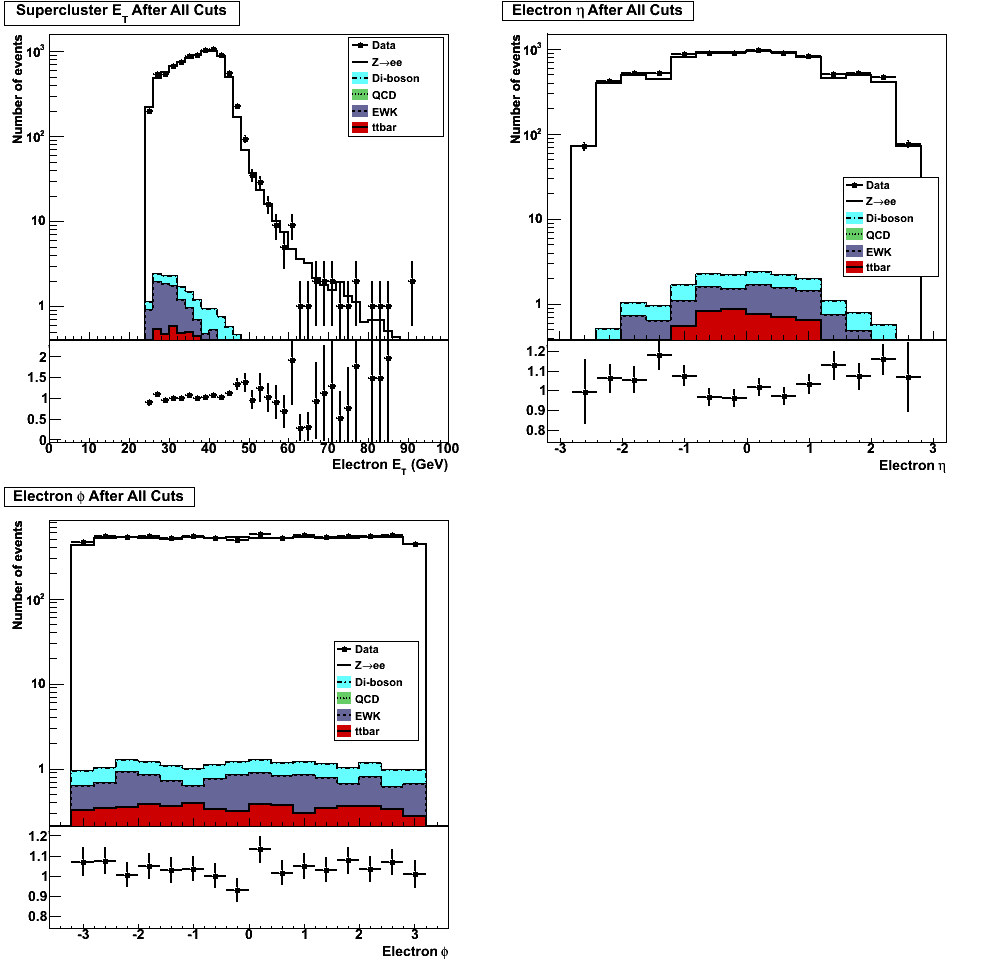
\includegraphics[width=180pt]{Figures/elecQuant-22Apr11.png}
%    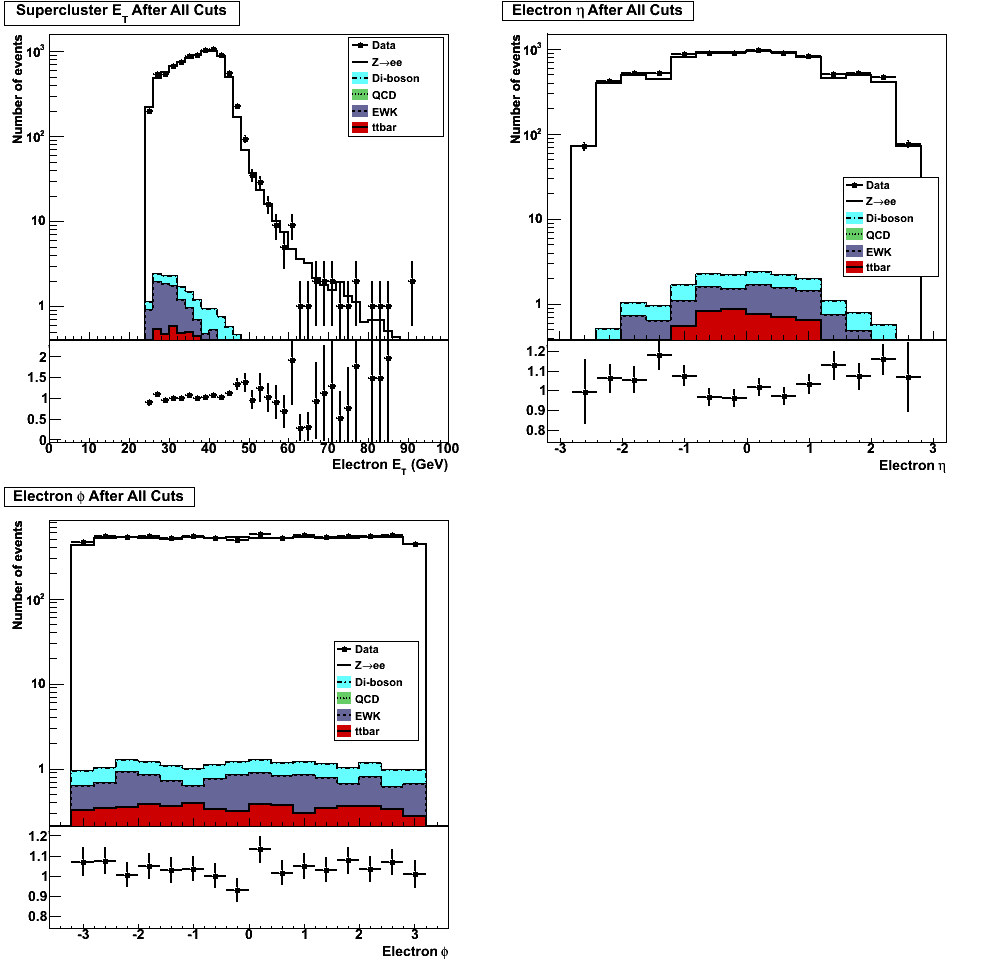
\includegraphics[width=360pt]{Figures/elecQuant-22Apr11.png}
    \subfloat[Transverse Energy]{\label{fig:ElectronEtAfterCuts}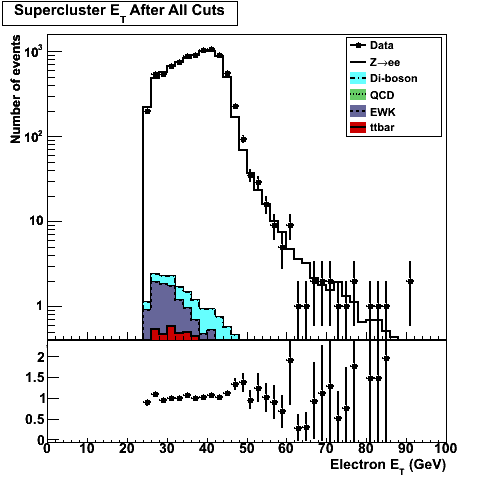
\includegraphics[width=180pt]{Figures/elecScEt-18May11.png}}
    \subfloat[Pseudorapidity]{\label{fig:ElectronEtaAfterCuts}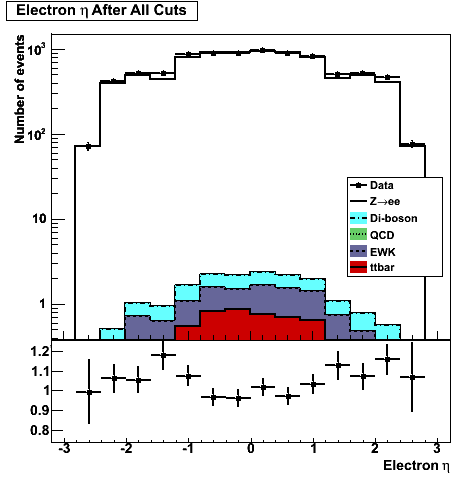
\includegraphics[width=180pt]{Figures/elecEta-18May11.png}}
    \subfloat[Azimuthal Angle]{\label{fig:ElectronPhiAfterCuts}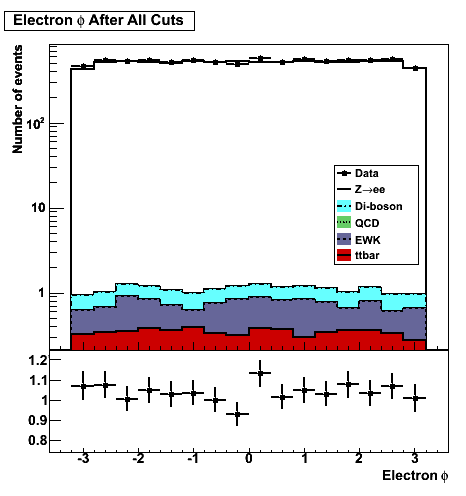
\includegraphics[width=180pt]{Figures/elecPhi-18May11.png}}
  \end{center}
%  \caption[Reconstructed electron/photon Pt, eta, phi spectra after ID]{Reconstructed electron/photon Pt, eta, phi spectra after ID.}
   \caption[\fixspacing Reconstructed electron \pt, $\eta$, $\phi$ spectra after full selection]{
   \fixspacing Spectra of reconstructed electron kinematic quantities after all electron selection cuts. 
   The plots show distributions for electron \pt, $\eta$, and $\phi$ respectively.  
   The agreement between real data and the simulated sample is good, demonstrating 
   that the effects of the cuts on the data are understood.  
  }
  \label{fig:RecoSpectraAfterEid}
 \end{figure}


%recap of invariant mass?

\section{Invariant Mass Spectrum} % DON'T REALLY NEED ALL EXPLANATORY STUFF HERE, IF IN INTRO CH???
\label{anMeth:invmass}
As explained in Section~\ref{theory:Zprod}, % it's done in introductory material
the invariant mass of a set of decay-product particles is 
%CONCEPTUAL EXPLANATION.
essentially the mass of the original particle that decayed. 
%to form the end-products.  
It is defined mathematically by %as 
\[
M_{inv}^2 = \left( \sum E \right)^2 - \left\| \sum \mathbf{p} \right\|^2
\]
where $ \mathbf{p} $ is the momentum 
and $ E $ the energy for a given particle; 
$ \sum $ denotes the sum over all particles 
-- a vector sum in the case of momentum, 
while $\left\| \mathbf{p} \right\|$ denotes the momentum's magnitude.  
In our case, for a two-particle system, this can be written as 
\[
M_{inv} = \sqrt{ \left(E_1 + E_2\right)^2 - \left\|\mathbf{p}_1 + \mathbf{p}_2\right\|^2 }
\]
The invariant mass distribution within the mass window 
for the electron pairs 
in the events surviving all selection cuts is shown in 
Fig.~\ref{fig:InvMass}.  
There are a total of 8453 data events in the plot, 
which makes up the total number of events passing 
the full event selection.  
An explanation of how the different simulation 
samples were combined can be 
found in Section~\ref{sim:MCSamples}.  
To combine data with Monte Carlo samples, 
the ratio of the data and Monte Carlo selection efficiencies, 
0.933 (taken from Table~\ref{TableEfficiencies}), 
was used as the scale factor.  
The peak around the Z mass (91 GeV) is clearly visible 
in both the Monte Carlo (solid) and data (points) distributions.  
The background contributions estimated from Monte Carlo simulation 
are shown as the colored (grayscale) areas.  
A slight shift in the peak position along the x-axis is 
evident, due to slight miscalibrations of 
the calorimeter response to given energies.  
This difference is accounted for in the 
systematic uncertainty due to the electron energy scale 
(see Section~\ref{anMeth:SystsOtherEleEScale}).  
The selected events are also divided into categories according 
to which part of the detector, barrel or endcap, 
each of their electron legs were located, 
and the resulting invariant mass spectra are 
shown in Fig.~\ref{fig:InvMassEtaDiv}.  
Agreement in each case is good to within the 
uncertainty.  

%ALSO TALK ABOUT HOW PLOTS SCALED??!!  
%somewhere, like in event selection? 
%I guess also in this section (different chapter)

%yield plot first, since this is what the rest is based on.  

%%Figures: Electron-pair invariant mass for trigger objects/ID only/ID+isolation, Fig. \ref{fig:InvMassAfterEachStep}
%Figures: Electron-pair invariant mass after full selection, Fig. \ref{fig:InvMass}

 \begin{figure}[htb]
  \begin{center}
    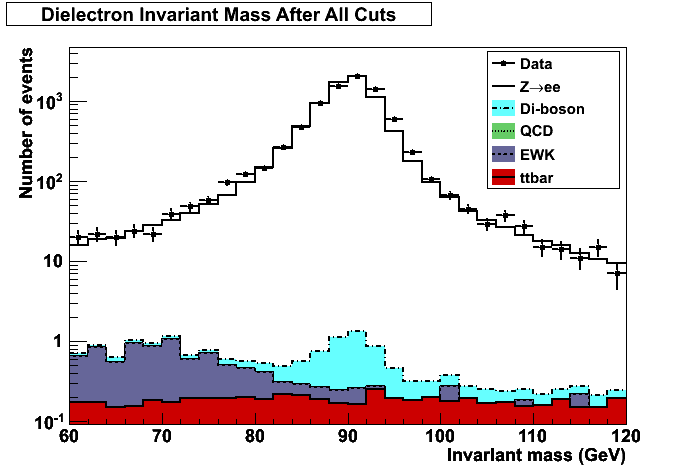
\includegraphics[width=360pt]{Figures/invMass-04Apr11.png}
  \end{center}
  \caption[\fixspacing Electron-pair invariant mass after full selection]
  {\fixspacing Electron-pair invariant mass after full selection.
    The peak around the Z mass (91 GeV) is clearly visible
    in both the Monte Carlo (solid) and data (points) distributions.
    The background contributions estimated from Monte Carlo simulation
    are shown as the colored (grayscale) areas.
    A slight shift in the peak position along the x-axis is
    evident, due to slight miscalibrations of
    the calorimeter response to given energies.
    This difference is accounted for in the
    systematic uncertainty due to the electron energy scale.
  }
  \label{fig:InvMass}
 \end{figure}

%Ooh, I do also have inv mass by eta plots

 \begin{figure}[htb]
  \begin{center}
%    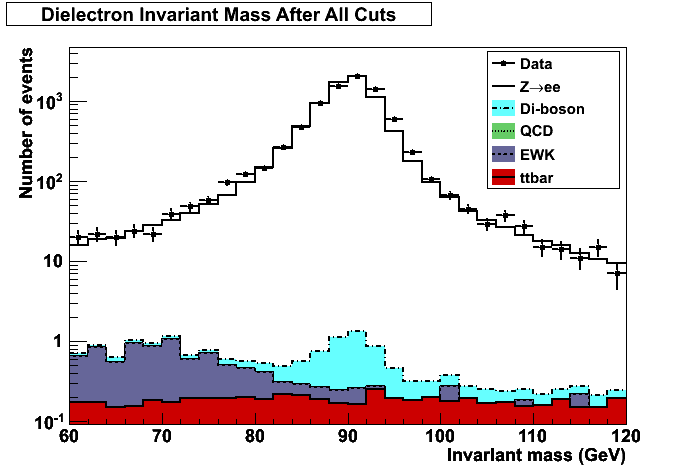
\includegraphics[width=360pt]{Figures/invMass-04Apr11.png}
    \subfloat[Barrel-barrel]{\label{fig:InvMassEtaDivBarrelBarrel}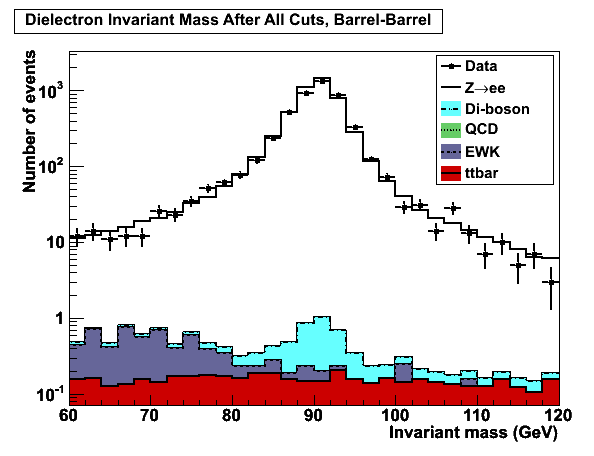
\includegraphics[width=180pt]{Figures/invMassEtaDiv-barrel-barrel-19May11.png}}
    \subfloat[Barrel-endcap]{\label{fig:InvMassEtaDivBarrelEndcap}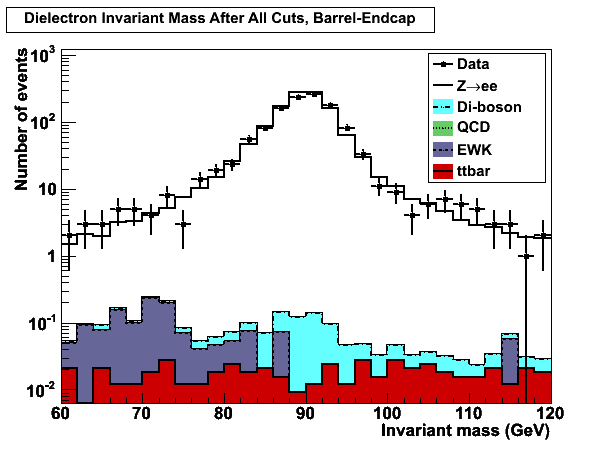
\includegraphics[width=180pt]{Figures/invMassEtaDiv-barrel-endcap-19May11.png}}
    \subfloat[Endcap-endcap]{\label{fig:InvMassEtaDivEndcapEndcap}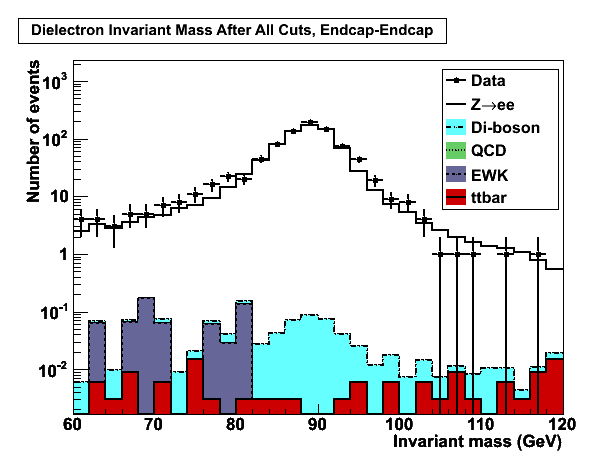
\includegraphics[width=180pt]{Figures/invMassEtaDiv-endcap-endcap-19May11.png}}
  \end{center}
  \caption[\fixspacing Electron-pair invariant mass by $\eta$]{
    \fixspacing Electron-pair invariant mass by $\eta$ after full selection.
    Each combination of electron $\eta$-positions is 
    distributed separately: 
    both electrons in the barrel 
    %(Fig.~\ref{fig:InvMassEtaDivBarrelBarrel}), 
    \subref{fig:InvMassEtaDivBarrelBarrel}, 
    one electron each in the barrel and the endcap 
    %(Fig.~\ref{fig:InvMassEtaDivBarrelEndcap}),
    \subref{fig:InvMassEtaDivBarrelEndcap},
    and both electrons in the endcap 
    %(Fig.~\ref{fig:InvMassEtaDivEndcapEndcap}).
    \subref{fig:InvMassEtaDivEndcapEndcap}.
    In each case the agreement between data and Monte Carlo simulation is good.  
  }
  \label{fig:InvMassEtaDiv}
 \end{figure}

% Also add plots for OS and SS??  Had them at one point!  
% WELL, last OS plot I have does not show good data/MC agreement

%% Figures: Same-sign dielectron invariant mass for electrons passing all selection steps, Fig. \ref{fig:SameSignInvMass}

%%  \begin{figure}[htb]
%%   \begin{center}
%%     
\includegraphics[width=360pt]{CMS-BW.pdf}
%%   \end{center}
%%   \caption[\fixspacing Same-sign dielectron invariant mass for electrons passing all selection steps]{\fixspacing Same-sign dielectron invariant mass for electrons passing all selection steps.}
%%   \label{fig:SameSignInvMass}
%%  \end{figure}



%\subsubsection{Distribution of Z Kinematic Variables} 
\section{Distributions of Z Kinematic Variables} % MOVED HERE 
%\label{evSel:Zquants}
\label{res:Zquants}
%Some amount of text explaining what this is for!  
Since a significant number of \Zee candidate events have been identified, 
it is useful to examine the kinematic properties of these events.  
Even though this analysis does not depend on these properties, 
comparing the distributions from the data with those from the simulated samples 
can provide an additional check of validity of the simulation.  

Fig. \ref{fig:Zquantities} shows the distributions of standard kinematic 
variables for the reconstructed Z candidates: transverse momentum, rapidity, and azimuthal angle. 
The data (black dots) is compared with the simulation including 
background samples (lines/filled areas).  
As the ratio plots show, the agreement is good in general; 
large error bars indicate bins where the event count is not 
high enough to give a very precise estimate 
(such as the higher range of the Z \pt plot).  
However, there are areas in which there is an evident discrepancy 
between the data and the simulation, 
most notably along the outer edges of the Z rapidity plot.  
Possible causes might include a slightly inaccurate description of the particle 
interaction in the generator, 
or a slight miscalibration of the detector.  
Since the difference is slight and does not affect this analysis, though, 
it can safely be ignored and the general agreement accepted.  

%Dude, what else to say here?  

 \begin{figure}[htb]
  \begin{center}
%    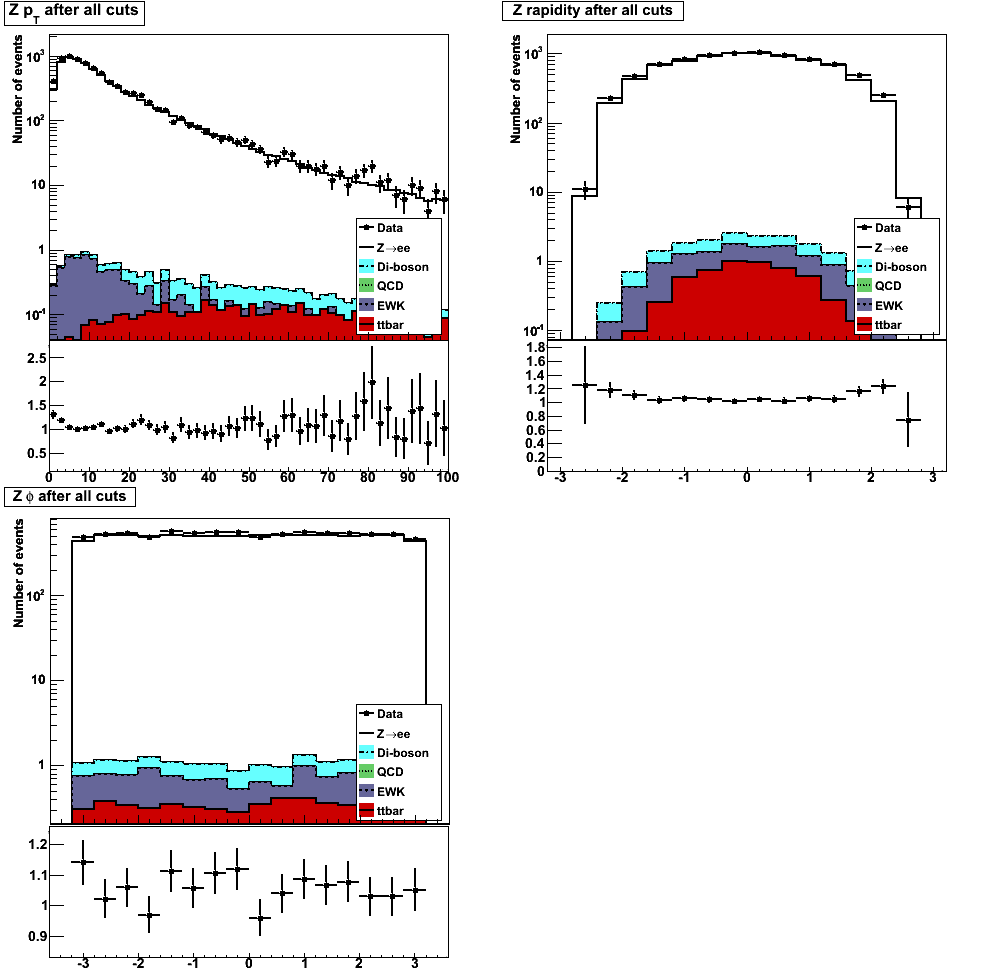
\includegraphics[width=360pt]{Figures/Zquantities-04Apr11.png}
    \subfloat[Transverse Momentum]{\label{fig:ZPt}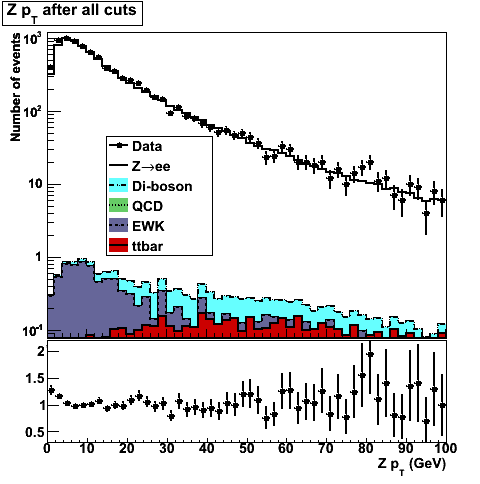
\includegraphics[width=180pt]{Figures/Zpt-18May11.png}}
    \subfloat[Rapidity]{\label{fig:ZRap}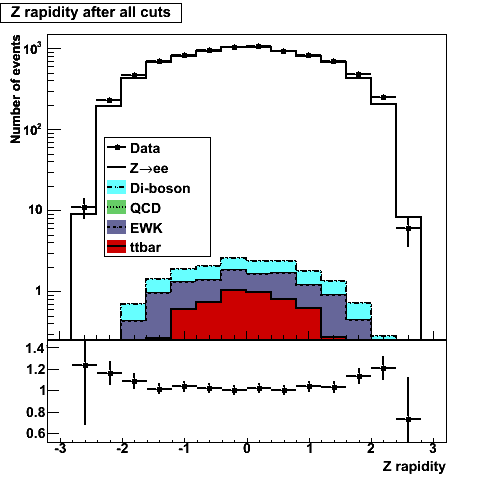
\includegraphics[width=180pt]{Figures/Zrap-18May11.png}}
    \subfloat[Azimuthal Angle]{\label{fig:ZPhi}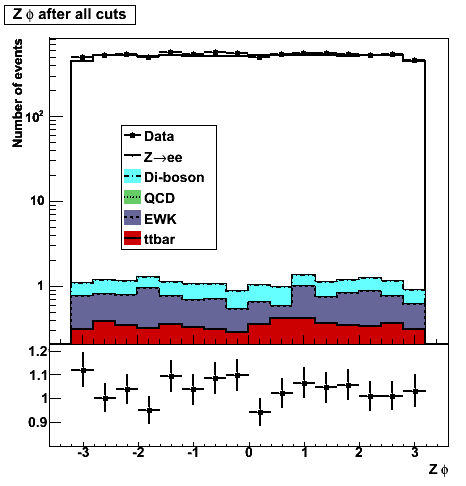
\includegraphics[width=180pt]{Figures/Zphi-18May11.png}}
  \end{center}
  \caption[\fixspacing Kinematic quantities of Z candidates after full selection]{
  \fixspacing Kinematic quantities of Z candidates after full event selection.
  }
  \label{fig:Zquantities}
 \end{figure}



\section{Cross Section Measurement}
\label{res:xsec}
%Cross section calculation: the table of numbers, 
%and the formula

As explained in Section~\ref{over:xsec}, 
the interaction cross section is calculated from the formula 
\[
\sigma \times \mathrm{BR} 
= \frac{\left( n_{total} - n_{background }\right)}{\mathcal{ L } \times \epsilon \times A }
\]
in which $n_{total}$, $n_{background}$, $\mathcal{ L }$, $\epsilon$, and $A$  
have been 
%measured 
determined 
experimentally.  
The measured values for these quantities 
are given in Table~\ref{TableXsecNumbers}. 

\begin{table}[htbp]
%  \centering
  \begin{center}
    \caption{\fixspacing Quantities used to calculate cross section.}
    \label{TableXsecNumbers}
%    \begin{tabular}[]{ | l | c | c | }
    \begin{tabular}[]{ | l | c | }
      \hline
      Quantity & Value \\ \hline \hline
      Luminosity $\mathcal{L}$ & 36.1 pb$^{-1}$ \\ \hline
      $n_{total}$ & 8453 \\ \hline
      $n_{background}$ & 19 \\ \hline
      Efficiency $\epsilon$ & 0.610 \\ \hline
      Acceptance $A$ & 0.387 \\ \hline
    \end{tabular}
  \end{center}
\end{table}



Plugging the values into the formula gives 
990 pb for the cross section.  
%
The sources of error in the measurement 
(see Section~\ref{anMeth:SystsSummary}) 
add a relative uncertainty of 4.8\%, 
corresponding to 48 pb, for a final result of 
\[
\sigma(p \bar{p} \rightarrow Z/\gamma *) \times \mathrm{BR}(Z \rightarrow e^+ e^- )
= 990 \pm 40 \mathrm{(lumi)} \pm 11 \mathrm{(stat)} \pm 17 \mathrm{(theory)} \pm 17 \mathrm{(syst)} \mathrm{pb} 
\]



\section{Comparison to Theory}
\label{res:theory}

To facilitate comparison of the cross section 
with theory, 
the CMS collaboration prepared a ``standard'' 
theoretical cross section value with FEWZ 
(see Section~\ref{sim:MCGensOther}), 
using the appropriate detector boundaries 
for the acceptance.  
The corresponding value obtained was 
972 $\pm$ 40 pb.  
The experimental value, 990 $\pm$ 48 pb, 
agrees with the theoretical value within 
the errors on both values 
(the difference is 1.9\% relative 
to the theoretical value).  

%number from FEWZ, errors.  how experimental number compares within errors

\section{Comparison to Other Experiments}
\label{res:prev}

%official CMS number, 

The official CMS vector boson cross section analysis 
\cite{CMSWZ}  
calculated a value of 992 pb.  
The official CMS analysis was very similar 
to this one, 
so it is expected that the numbers should 
agree very closely.  
The difference between them comes to 0.2\%.  

The ATLAS collaboration also performed an analysis 
of the vector boson production cross sections 
\cite{ATLASZ}. 
The selection criteria were slightly different 
from those used in CMS: 
the electron $\eta$ range used was 
$|\eta| < 1.37, 1.52 < |\eta| < 2.47$, 
the electrons were required to have a 
transverse energy of 20 GeV instead of 25, 
and the invariant mass range was 66 to 116 GeV 
instead of 60 to 120 GeV.  
Nevertheless, the analyses are comparable.  
The \Zee cross section obtained by ATLAS is 
\[
\sigma(p \bar{p} \rightarrow Z/\gamma *) \times \mathrm{BR}(Z \rightarrow e^+ e^- )
= 972 \pm 33 \mathrm{(lumi)} \pm 10 \mathrm{(stat)} \pm 38 \mathrm{(theory)} \pm 34 \mathrm{(syst)} \mathrm{pb} 
\]
This compares well with the number obtained 
in this analysis, 
as well as with the official CMS result.  

%tevatron numbers??  doesn't really add anything

%ADD FUN PLOTS, like move inv mass here?? 
%also Z quantity plots. 
%and do I have electron distributions somewhere? 
%YES, they're in evSel.  along with Z distro plots.  
%Those are really sort of results, I should put them there! 

\clearpage